\documentclass[a4paper, 12pt]{article}

\usepackage{cmap}
\usepackage[utf8]{inputenc}
\usepackage[T2A]{fontenc}
\usepackage[english, russian]{babel}
\usepackage{graphicx}
\DeclareGraphicsExtensions{.pdf, .png, .jpg}
\usepackage{amsmath}
\usepackage{tikz}
\usetikzlibrary{shapes, arrows}
\usepackage{url}
\usepackage{}
\usepackage[colorlinks = true,
linkcolor = black,
urlcolor = blue,]{hyperref}
\usepackage[left=2cm,right=2cm,top=2cm,bottom=2cm,bindingoffset=0cm]{geom
etry}
\usepackage{multirow}

\author{Мелехов Артём ПВ-223}
\title{LaTeX}
\date{\today}



\begin{document}

\maketitle

\newpage

\section{\centering Текст}

\begin{flushleft}
\textit{
Послушайте!\\
Ведь, если звезды зажигают --\\
значит -- это кому-нибудь нужно?\\
Значит -- кто-то хочет, чтобы они были?\\
Значит -- кто-то называет эти плево́чки жемчужиной?
}
\end{flushleft}

\begin{flushright}
\textit{
И, надрываясь\\
в метелях полу́денной пыли,\\
врывается к богу,\\
боится, что опоздал,\\
плачет,\\
целует ему жилистую руку,\\
просит --\\
чтоб обязательно была звезда! --\\
клянется --\\
не перенесет эту беззвездную муку!
}
\end{flushright}

\begin{flushleft}
\textit{
А после\\
ходит тревожный,\\
но спокойный наружно.\\
Говорит кому-то:\\
<<Ведь теперь тебе ничего?\\
Не страшно?\\
Да?!>>
}
\end{flushleft}

\begin{flushright}
\textit{
Послушайте!\\
Ведь, если звезды\\
зажигают --\\
значит -- это кому-нибудь нужно?\\
Значит -- это необходимо,\\
чтобы каждый вечер\\
над крышами\\
загоралась хоть одна звезда?!\\
}
\end{flushright}

\section{\centering Картинка}
\begin{figure}[h]
    \centering
    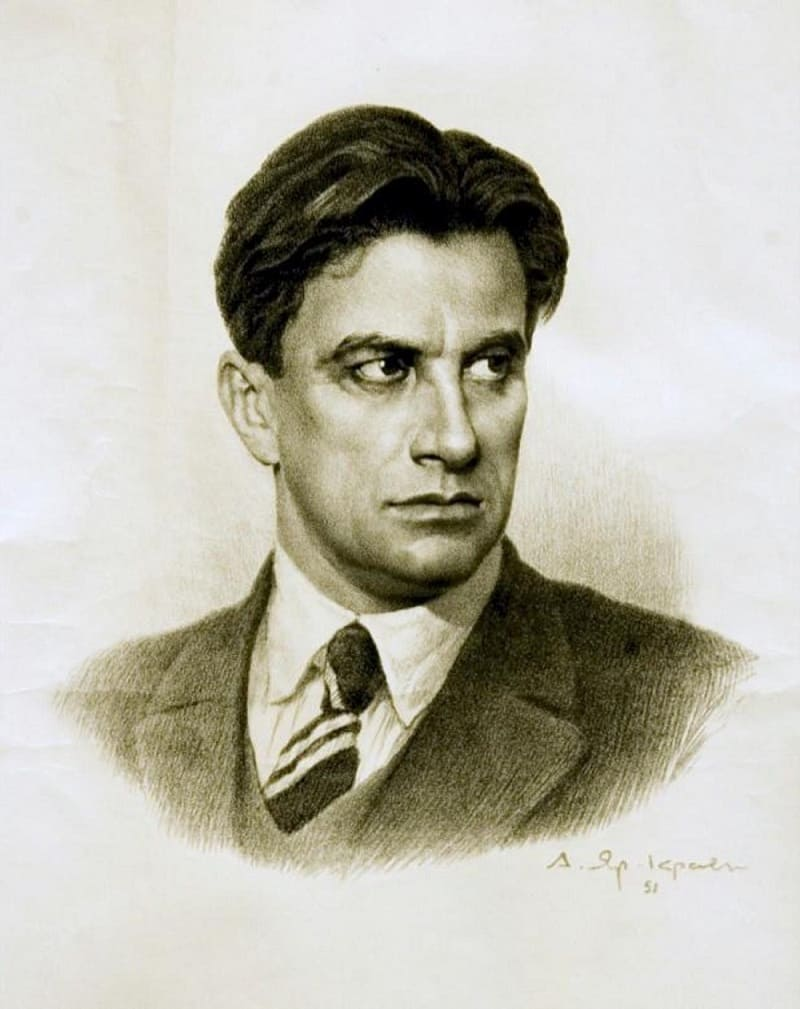
\includegraphics{vladimir_mayakovskiy.jpg}
    \caption{Владимир Маяковский}
    \label{fig:AutorFace}
\end{figure}

\newpage
\textbf{Люимые произведения Маяковского:}
\begin{itemize}
    \item Послушайте!
    \item <<Ешь ананасы, рябчиков жуй...>>
    \item Утро
    \item А вы могли бы?
    \item Адище города
\end{itemize}

\newpage
\section{\centering Математические формулы}
Система уравнений:
\begin{equation*}
 \begin{cases}
   x = 3y * 18,
   \\
   y = 27x
 \end{cases}
\end{equation*}
Возведение в степень:
\[ x^2 \]
Интеграл:
\[ \int_{0}^{n} x \]
Сигма (сумма):
\[ \sum_{n=1}^{\infty} x = \infty \]
Дробь:
\[ \frac {1} {42} \]

\newpage

\begin{tikzpicture}

\tikzstyle{connector} = [draw, -latex']
\tikzstyle{terminator} = [rectangle, draw, text centered, rounded corners, minimum height=2em]
\tikzstyle{process} = [rectangle, draw, text centered, minimum height=2em]
\tikzstyle{decision} = [diamond, draw, text centered, minimum height=2em]
\tikzstyle{data}=[trapezium, draw, text centered, trapezium left angle=60, trapezium right angle=120, minimum height=2em]

\node at (0, 0) [terminator] (start) {Начало};
\node [data] at (0,-2) (data_in) {Ввод};
\node [data] at (0,-4) (data_out) {Ввод};
\node [decision] at (0,-6.5) (is_right) {Проверка};
\node [process] at (4,-6.5) (p1) {Процесс1};
\node [process] at (0,-9) (p2) {Процесс2};
\node [decision] at (0,-11.5) (cycle) {Цикл};;
\node [process] at (-3,-14) (p3) {Процесс3};
\node at (3, -16) [terminator] (end) {Конец};

\node[draw=none] at (1.5, -6) (no) {};
\node[draw=none] at (0.5, -8) (yes) {+};

\node[draw=none] at (1.5, -11) (no) {};
\node[draw=none] at (0.5, -12.5) (yes) {+};

\path [connector] (start) -- (data_in);
\path [connector] (data_in) -- (data_out);
\path [connector] (data_out) -- (is_right);
\path [connector] (is_right) -- (p1);
\path [connector] (is_right) -- (p2);
\path [connector] (p2) -- (cycle);
\path [connector] (cycle) |- (p3);
\path [connector] (p3) |- (cycle);;
\path [connector] (p1) |- (end);
\path [connector] (cycle) -| (end);

\end{tikzpicture}

\newpage
\begin{center}
    \begin{table}
\caption{Аттестационная ведомость группы ПВ-223}
\begin{tabular}{|c|c|c|c|c|c|c|c|c|c|c|c|c|c|}
\hline
\multirow{2}{*}{№} &
\multirow{2}{*}{ФИО студента} &
\multicolumn{2}{|c|}{Пропуски} &
\multicolumn{9}{|c|}{Дисциплины} &
\multirow{2}{*}{\rotatebox{90}{Среднее значение}} \\ \cline{3-13}
& &
Ув. &
Не ув. &
\rotatebox{90}{Алг. и геом.} &
\rotatebox{90}{Введ. в проф.} &
\rotatebox{90}{Ин. яз.} &
\rotatebox{90}{Информатика.} &
\rotatebox{90}{КР и дел. общ.} &
\rotatebox{90}{Мат. анализ.} &
\rotatebox{90}{ОП} &
\rotatebox{90}{ЭДФКС} &
\rotatebox{90}{Физика} & \\
\hline
1 & Мелехов Артём Дмитриевич &
0 & 42 &
2 & 2 & 2 & 2 & 2 & 2 & 2 & 2 & 2 & 2 \\
\hline
2 & Мелехов Дмитрий Артёмович &
0 & 0 &
5 & 5 & 5 & 5 & 5 & 5 & 5 & 5 & 5 & 5 \\
\hline
3 & Артёмов Мелех Дмитриевич &
0 & 0 &
5 & 5 & 5 & 5 & 5 & 4 & 4 & 5 & 4 & 5 \\
\hline
4 & Артёмов Дмитрий Мелехович &
40 & 0 &
4 & 4 & 2 & 3 & 4 & 5 & 5 & 5 & 4 & 2 \\
\hline
5 & Дмитриев Мелех Артёмович &
0 & 0 &
5 & 5 & 5 & 5 & 5 & 5 & 5 & 5 & 5 & 5 \\
\hline
\multicolumn{4}{|c|}{Среднее значение} &
5 & 5 & 5 & 5 & 5 & 5 & 5 & 5 & 5 & 5\\
\hline
\end{tabular}
\end{table}
\end{center}


\newpage

\def\figurename{Рис.}

% Титульный лист

\begin{title}
\newpage
\thispagestyle{empty}
\begin{center}
МИНИСТЕРСТВО НАУКИ И ВЫСШЕГО ОБРАЗОВАНИЯ \\
РОССИЙСКОЙ ФЕДЕРАЦИИ
\end{center}
\vfil
\begin{center}\small
ФЕДЕРАЛЬНОЕ ГОСУДАРСТВЕННОЕ БЮДЖЕТНОЕ ОБРАЗОВАТЕЛЬНОЕ УЧРЕЖДЕНИЕ
ВЫСШЕГО ОБРАЗОВАНИЯ
\end{center}
\vfil
\begin{center}\textbf{
«БЕЛГОРОДСКИЙ ГОСУДАРСТВЕННЫЙ
ТЕХНОЛОГИЧЕСКИЙ УНИВЕРСИТЕТ им. В. Г. ШУХОВА» \\
(БГТУ им. В.Г. Шухова)
}\end{center}
\vfil
\begin{center}\small
Кафедра программного обеспечения вычислительной техники и
автоматизированных систем
\end{center}
\vfill
\begin{center}
\textbf{Индивидуальное домашнее задание №1} \\
по дисциплине: Информатика \\
тема: «Криптографические методы защиты информации»
\end{center}
\vfill
\begin{tabularx}{\textwidth} {
&
Выполнил: ст. группы ПВ-223 \\
Мелехов Артём Дмитриевич
}
\end{tabularx}
\begin{center}
\vfill
Белгород 2022 г.
\end{center}
\end{title}


% Оглавление

\newpage
\renewcommand\contentsname{Оглавление}
\tableofcontents

% Введение

\newpage
\section*{Введение}\addcontentsline{toc}{section}{Введение}

% Основная часть

\newpage
\section{Основная часть}
\subsection{Основная часть 2}

% Заключение
\newpage
\section*{Заключение}\addcontentsline{toc}{section}{Заключение}

% Список использованной литературы

\newpage

\section*{Список использованной
литературы}\addcontentsline{toc}{section}{Список использованной
литературы}
\begin{itemize}
\item Электронный ресурс: <<YouTube>> \\
\url{https://youtu.be/yZeGuTpsv0I}
\end{itemize}

% Конец документа

\end{document}